\documentclass[../../main.tex]{subfiles}
\begin{document}
\chapter{Multi-Track and Non-Linear Synthesis}
\label{ch:multi_track}

Human movement is a symphony of coordinated actions, where each part of the body plays a distinct role, yet all work together in harmony to create a seamless expression of intent. The essence of this coordination lies in the ability to perform multiple actions simultaneously or in carefully timed sequences, with each movement contributing to the larger tapestry of physical expression. Traditional approaches to understanding or replicating this complexity often fall short, reducing human motion to a linear series of bone rotations that lack the depth and nuance of true human movement.

The concept of multi-track control offers a different perspective—one that acknowledges the layered nature of our physical existence. It recognizes that our movements are not isolated but interwoven, with each gesture or posture influencing and being influenced by others. By allowing multiple threads of action to unfold concurrently or in precise intervals, multi-track control mirrors the natural rhythm and flow of life. It captures the interplay between stillness and motion, the balance of tension and release, and the silent dialogue between different parts of the body as they move together yet independently. In doing so, it brings us closer to understanding the profound complexity of human movement, honoring the subtlety and grace inherent in every action.

Similarly, non-linearity in movement reflects the dynamic and adaptive nature of human actions. Just as life rarely follows a straightforward path, our movements often involve layers of simultaneous actions that interact in complex ways. In fields like video editing or film production, non-linear control allows creators to work with multiple layers of footage, sounds, and effects, enabling them to craft scenes where various elements unfold together, contributing to a richer and more cohesive narrative.

In the realm of sign language, the non-linear and multi-track nature of human movement is particularly evident. Sign language involves a combination of simultaneous gestures, facial expressions, and body movements, all working together to convey meaning. By adopting a non-linear, multi-track approach, we can more accurately capture the intricate coordination involved in signing, where gestures and expressions occur in parallel, influencing and overlapping with each other. This approach respects the complexity and interconnectivity inherent in sign language, allowing for a more nuanced and realistic portrayal of its dynamic and expressive nature. In doing so, it brings us closer to truly understanding and representing the fluidity and richness of sign language as it is naturally used, honoring its depth and complexity as a form of human communication.

This chapter aims to present a novel approach to sign language synthesis using multi-track and non-linear editing techniques. It showcases improvements in animation quality and flexibility, demonstrating how these techniques preserve the dynamics of individual animation blocks and enhance procedural generation capabilities.

The content of this chapter is structured as follows: todo

\section{Related Work}
\label{sec:related_work}

Both multi-track and non-linear editing have been widely used in various fields, including film production, video editing(figure \ref{fig:video_edit}), and animation (figure \ref{fig:nle_blender}). 

\begin{figure}[h]
    \centering
    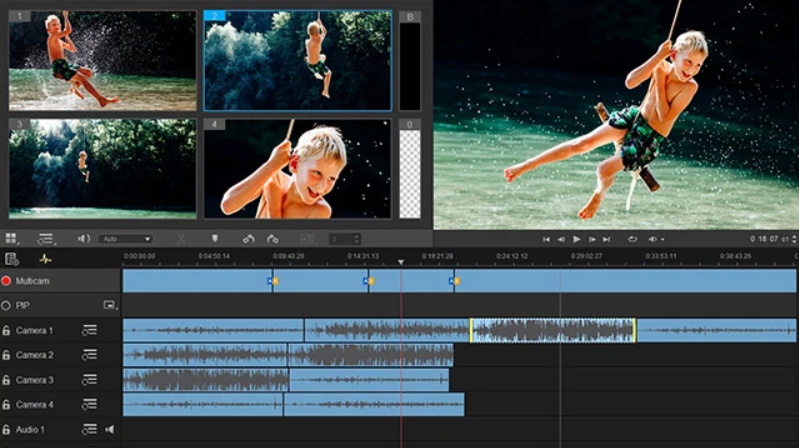
\includegraphics[width=0.8\textwidth]{chapters/multi_track/images/video_editing.jpg}
    \caption{Video editing software interface showing multiple tracks for editing video and audio clips.}
    \label{fig:video_edit}
\end{figure}

\begin{figure}[h]
    \centering
    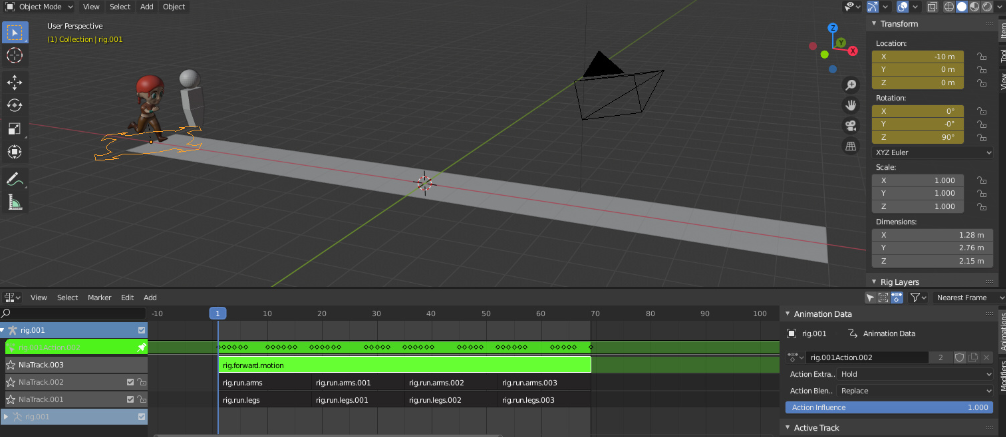
\includegraphics[width=0.8\textwidth]{chapters/multi_track/images/nle_blender.jpg}
    \caption{Blender's non-linear editor interface showing multiple tracks for editing animation clips.}
    \label{fig:nle_blender}
\end{figure}

However, their appliations in both procedural animation and sign language synthesis are limited.

\subsection{Existing low-level AZee synthesizor}
\label{subsecc:old_azee_synthesizor}

Although AZee is multi-track by nature (where the lingusit has the ability to crate the track), the low-level AZee synthesizor is based on a flattened \emph{AnimatedScore} representation that flattenes each track made by the linguist. This flattening layer loses the multi-track information and the dynamics of the original AZee description. 

For example, consider the following low-level AZee description:

\begin{verbatim}
    todo
\end{verbatim}

This description when compiled with the AZee interpreter generates an AZee \emph{SyncedScore} using the algorithm \ref{alg:azee_recursion} \cite{todo} that is show in in figure \ref{fig:azee_synced_score}.

\begin{figure}[h]
    \centering
    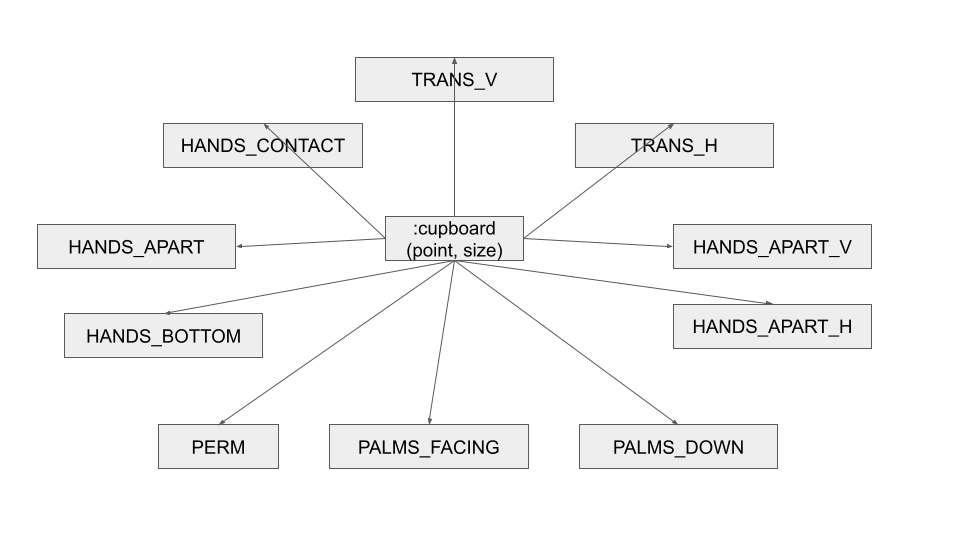
\includegraphics[width=0.8\textwidth]{chapters/multi_track/images/azee_synced_score.png}
    \caption{AZee Synced Score generated from the low-level AZee description.}
    \label{fig:azee_synced_score}
\end{figure}

Figure \ref{fig:azee_flattened_score} shows the flattened version of this AZee Synced Score, where all the tracks are merged into a single track. This flattening is done by collecting all the constraints for each frame and applying them to the corresponding bone rotations during animation.

This approach is also inextensible to be used with pre-animated motion data since the flattened representation does not contain the original location of the corresponding animation block on the timeline. 

\subsection{Paula}
\label{subsec:paula}

On the contrary, a multi-track approach to sign language synthesis has already been done by \cite{todo}. Paula is a multi-track sign language synthesis system that strictly uses pre-recorded motion data. The system is based on a multi-track timeline where each track is created by the artist(or can be based on the AZee description). The Paula interface is shown in figure \ref{fig:paula}.

\begin{figure}[h]
    \centering
    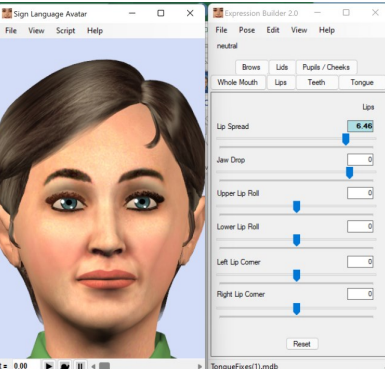
\includegraphics[width=0.8\textwidth]{chapters/multi_track/images/paula.png}
    \caption{Paula interface showing a multi-track timeline for sign language synthesis.}
    \label{fig:paula}
\end{figure}

However, Paula doesn't support low-level synthesis from AZee descriptions. This poses a challenge in scalability since an artist is always needed to create the building blocks of the animation. Although, the interface is tailored specifically for creating sign language content, a human intervention is still needed. Another drawback of Paula is that it is based on a single avatar model, which limits the diversity of the animations that can be created.

\subsection{Outside Sign Language Synthesis}
\label{subsec:other_multi_track}

The concept of multi-track timeline control for text-driven 3D human motion generation was also explored by \cite{petrovich24stmc}. The work introduces a novel way to address the limitations of previous methods that lacked fine-grained control over action composition and timing. This approach allows users to define multiple textual prompts within overlapping temporal intervals, enabling precise control over complex actions (figure \ref{fig:multi_track_other}). The proposed Spatio-Temporal Motion Collage (STMC) method, which operates at test-time, integrates with pre-trained motion diffusion models to generate realistic motions that adhere to the specified timeline. However, it is not for use in sign language synthesis, where precise and context-sensitive hand and body gestures are required, as it relies heavily on models not specifically designed for such detailed tasks.

\begin{figure}
    \centering
    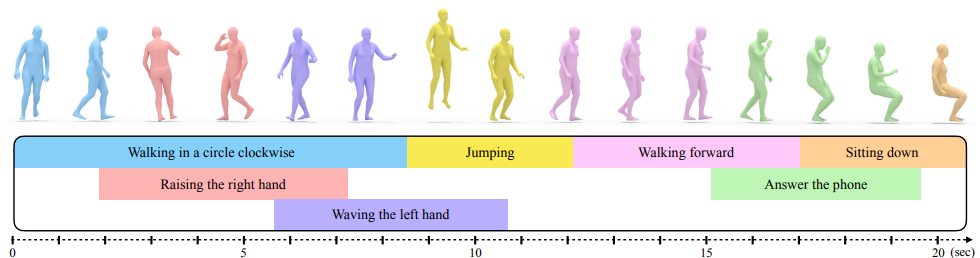
\includegraphics[width=0.8\textwidth]{chapters/multi_track/images/multi_track_other.png}
    \caption{Multi-track timeline control for text-driven 3D human motion generation.}
    \label{fig:multi_track_other}
\end{figure}

\section{AZee Synced Score to Multi-Track Timeline}
\label{sec:score_to_timeline}

One of the areas which this work aims to address is the direct creation of a multi-track animation timeline from a multi-track AZee Synced Score. This approach allows for the preservation of the original multi-track information and dynamics present in the AZee description. The algorithm \ref{alg:azee_timeline} shows how the AZee Synced Score is converted into a multi-track timeline.

\begin{algorithm}
    \caption{AZee Recursion Algorithm (Simplified)}
    \label{alg:azee_timeline}
    \begin{algorithmic}[1]
        \Function{CreateBlocks}{name, score, parent\_name, parent\_score, dynamic\_points}
            \If {parent\_score is not None}
                \State name $\gets$ name + "." + parent\_name
                \State \Call{UpdateSyncRules}{parent\_score, name}
            \EndIf
            
            \State \Call{UpdateBlockTimings}{name, score, parent\_name, parent\_score}
            \If {score.dynamic\_point}
                \State dynamic\_points.append(score.dynamic\_point)
            \EndIf
            
            \If {shortcut\_action $\gets$ \Call{GetShortcutAction}{score} \textbf{and} UseShortcutActions()}
                \State \Return \Call{CreateShortcutBlock}{name, score, parent\_score}
            \ElsIf {score is a SyncedScore}
                \For {child\_name, child\_score in score.block\_contents}
                    \State \Call{CreateBlocks}{child\_name, child\_score, name, score, dynamic\_points}
                \EndFor
            \Else
                \State \Return \Call{CreateRegularBlock}{name, score, parent\_score}
            \EndIf
            
            \If {parent\_score is not None}
                \State \Call{UpdateParentTimings}{parent\_name, name}
            \EndIf
        \EndFunction
    \end{algorithmic}
\end{algorithm}

The figure \ref{fig:azee_timeline} shows the multi-track timeline generation for a simple example.

\begin{figure}[h]
    \centering
    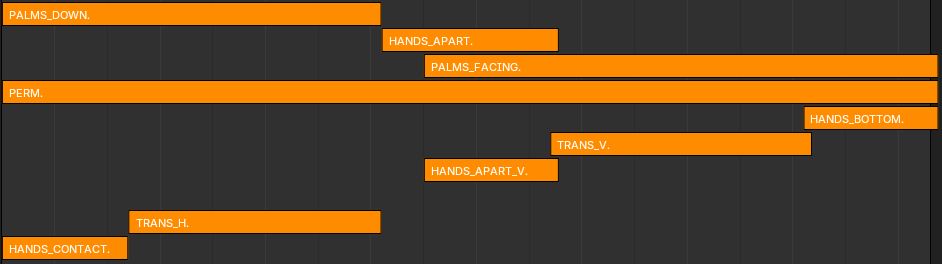
\includegraphics[width=0.8\textwidth]{chapters/multi_track/images/azee_timeline.png}
    \caption{Multi-track timeline generation from an AZee Synced Score.}
    \label{fig:azee_timeline}
\end{figure}

\section{AZee and Non-Linearity}
\label{sec:azee_nl}

The order of synthesis of the blocks in the multi-track timeline is crucial for avoiding conflicts and ensuring the correct execution of constraints. Thus, an action which happens later in the timeline might be synthesized first. This makes the synthesis non-linear. Figure \ref{fig:example_azee_non_linear} shows an example of non-linear synthesis.

\begin{figure}[h]
    \centering
    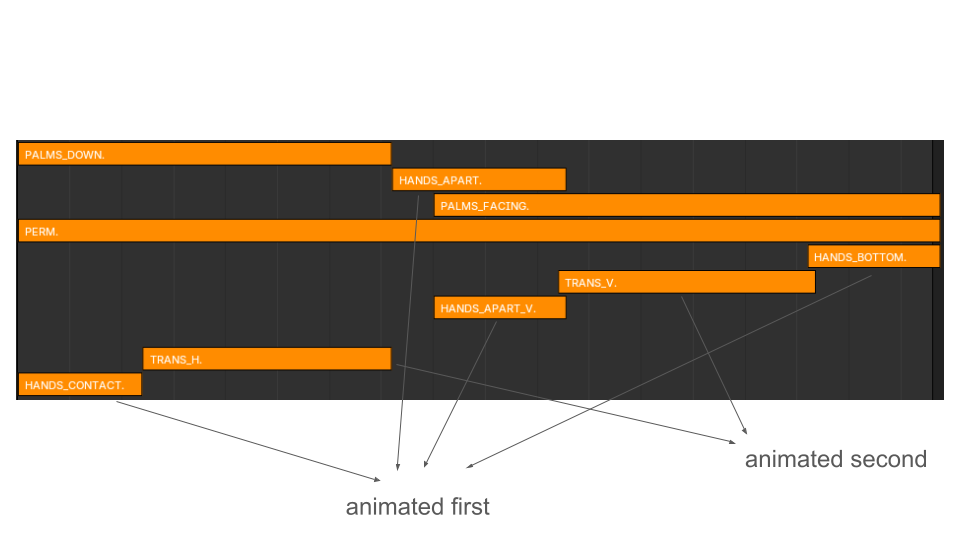
\includegraphics[width=0.8\textwidth]{chapters/multi_track/images/example_azee_non_linear.png}
    \caption{Example of non-linear synthesis in AZee.}
    \label{fig:example_azee_non_linear}
\end{figure}

\section{Resolving Block Conflicts}
\label{sec:resolve_conflitcs}

Since the blocks in the multi-track timeline can have constraints that affect the same body parts, conflicts can arise. These conflicts need to be resolved to ensure the correct execution of the constraints. The following rules are used to resolve conflicts:

\subsection{Timely Evaluation}
\textbf{Problem:} Overlapping blocks with different start times.
\textbf{Solution:} Evaluate blocks chronologically to maintain logical sequence.

\subsubsection{Rule 2: Constraint Precedence}
\textbf{Problem:} Overlapping blocks starting simultaneously.\\
\textbf{Solution:} Give precedence to placement constraints over orientation constraints.

\subsubsection{Rule 3: Second Pass for Transpaths}
\textbf{Problem:} Blocks with transpath constraints.\\
\textbf{Solution:} Evaluate these blocks in a second pass after other constraints are resolved.

\subsubsection{Rule 4: Second Pass for Holds}
\textbf{Problem:} Blocks with hold constraints.\\
\textbf{Solution:} Evaluate these blocks in a second pass to ensure dependent constraints are maintained.

\subsection{Pre-animated blocks}
\textbf{Problem:} Overlapping blocks with different start times.\\
\textbf{Solution:} Evaluate blocks chronologically to maintain logical sequence.

Cases where blocks do not overlap or affect different bone chains can be evaluated independently. This includes non-overlapping blocks and constraints such as morph and look, which act independently from other constraints.


\ection{Pre-animated blocks}
\label{sec:preanim_blocks}
todo

\section{Block Ordering}
\label{sec:block_ordering}


\section{Implementation and Results}
\label{sec:implem_results}


The multi-track timeline is implementated in blender's non-linear editor. Each AZee Score, when animated, generates a blender action which is put on the non-linear editor as a block with duration specified by the AZee \emph{sync rules}

\section{Evaluation}
\label{sec:eval}

we dont evaluate sign language synthesis, we evaluate azee synthesis

against mediapipe 

against paula

against rosetta mocap

against state of the art and sgnify

Examples of synthesized AZee descriptions, comparing flattened and non-flattened synthesis. Highlight the preservation of dynamics and any potential issues encountered. Discuss the use of Frobenius distance as a metric for evaluating the accuracy of the synthesized animations.

\section{Conclusion}
Summarize the benefits of the proposed multi-track synthesis algorithm, emphasizing the preservation of dynamics and improved naturalness in sign language animations. Highlight the contributions of this approach to the field of sign language synthesis.

\end{document}
